\documentclass[4paper]{article}
\usepackage[spanish]{babel}
%\usepackage[ansinew]{inputenc}
\usepackage[utf8x]{inputenc}
%\usepackage[utf-8]{inputenc}
%\usepackage[T1]{fontenc}
\usepackage{graphicx}
\usepackage{multicol}
\usepackage{float}
%\usepackage{longtable}
%\usepackage{array}
%\usepackage{multirow}
%\usepackage[latin1]{inputenc}
%\inputencoding{latin}
\newcommand{\J}{JavaScript}
\newcommand{\s}{express}

%\newcommand{\j}{JavaScript }

\renewcommand{\tablename}{Tabla}
\renewcommand{\S}{Introducción a \s}
\author{Manuel Molino Milla}
\title{\textbf{\S}}
\date{\today}

\begin{document}
\maketitle 
\tableofcontents
\newpage

\section{Introducción}
\subsection{¿Qué es \s?}
\begin{itemize}
\item Es un framework para desarrollo web.
\item Facilita el desarrollo web con \emph{node.js}
\item Entre sus características están:
\begin{itemize}
\item Permite crear rutas en función de peticiones web o métodos HTTP.
\item Configura \emph{middlewares} a las peticiones web.
\item Permite renderizar dinámicamente HTML mediante argumentos pasados a plantillas.
\end{itemize}
\end{itemize}

\subsection{Instalación}
\begin{quote}
npm install express
\end{quote}
Instala localmente en el directorio \emph{node\_modules}
Es interesante acompañar \s ~ con otros módulos como:
\begin{description}
\item[body-parser] es un middleware para datos JSON, Raw, Text y URL encoded
\item[cookie-parser] para establecer \emph{cookies}
\end{description}
Y muchos mas.
\subsection{Hello World con \s}
\begin{verbatim}
var express = require('express');
var app = express();

app.get('/', function (req, res) {
   res.send('Hello World');
})

var server = app.listen(8081, function () {
   var host = server.address().address
   var port = server.address().port
   
   console.log("Example app listening at 8081")
})
\end{verbatim}

\section{Enrutador con \s}
\subsection{Ejemplo}
\begin{verbatim}
var express = require('express');
var app = express();
var bodyParser = require('body-parser');

// parse application/x-www-form-urlencoded 
app.use(bodyParser.urlencoded({ extended: false }))
 
// parse application/json 
app.use(bodyParser.json())
app.set('port', process.env.PORT || 3000);

app.get('/', function (req, res) {
     res.send('Hello World');
})

app.get('/users/:userName', function(request, response) {
     var name = request.params.userName;
     response.send('¡Hola, ' + name + '!');
});

app.post('/users', function(request, response) {
    var username = request.body.username;
    response.send('¡Hola, ' + username + '!');
});

//http://localhost:3000/personal/15
//http://localhost:3000/personal/edit/15
app.get(/\/personal\/(\d*)\/?(edit)?(\/(\d*))?/, function (request, response) {
    var message = 'el perfil del empleado #' + request.params[0];
    if (request.params[1] === 'edit') {
        message = 'Editando ' + message;
    } else {
        message = 'Viendo ' + message;
    }
    response.send(message);
});



var server = app.listen(app.get('port'), function () {
     var host = server.address().address
     console.log("Example app listening at http://%s:%s", host, app.get('port'))
})

\end{verbatim}
Usamos como cliente algún plugin para un navegador como puedes ser rest-client, postman o rested
\begin{figure}[H]
  \centering
    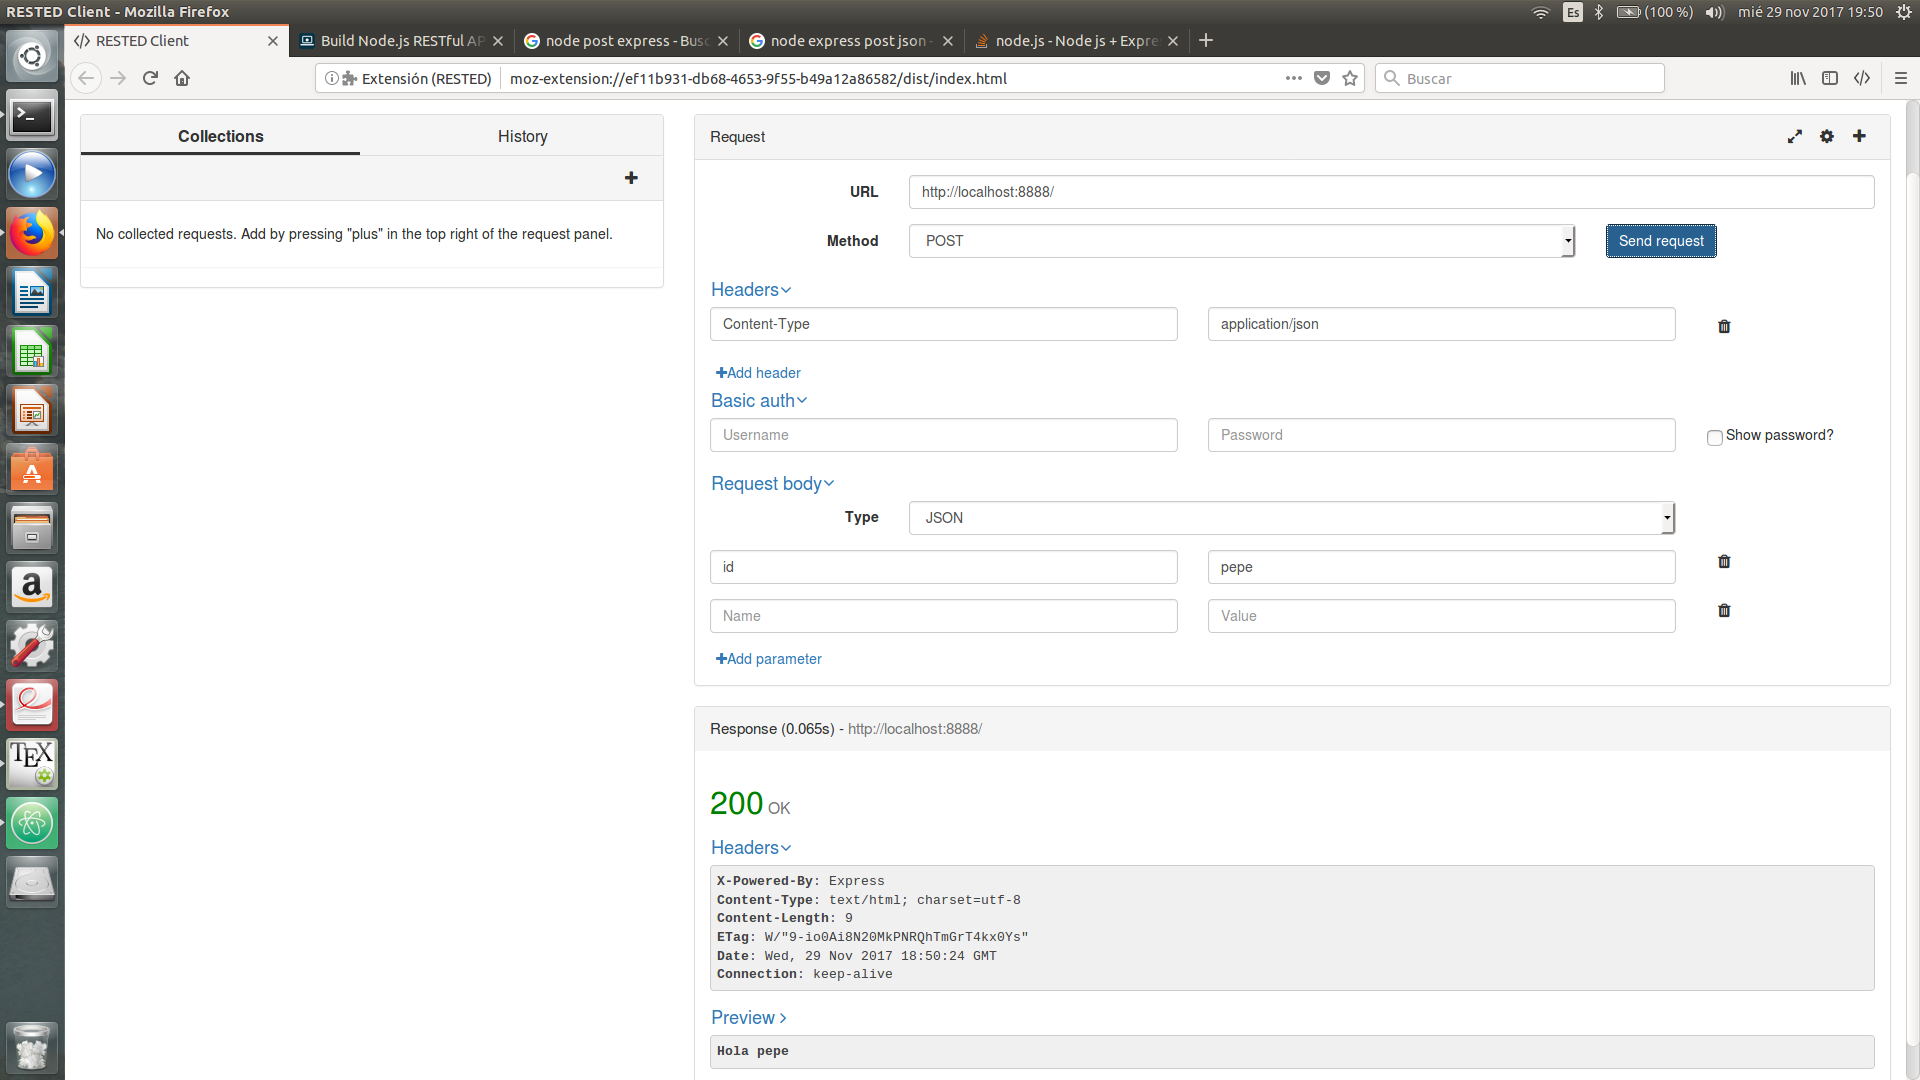
\includegraphics[scale=0.2]{post.png}
  \caption{RESTED Cliente}
  \label{fig:ejemplo}
\end{figure}
\newpage

\subsection{Sirviendo páginas estáticas}
Ejemplo \emph{index.html}
\begin{verbatim}
<html>
   <body>
     <form action = "http://127.0.0.1:8081/process_get" method = "GET">
        First Name: <input type = "text" name = "first_name">  <br>
        Last Name: <input type = "text" name = "last_name">
        <input type = "submit" value = "Submit">
     </form>
    </body>                                              
</html>
\end{verbatim}
Presentando y procesando el formulario:
\begin{verbatim}
var express = require('express');
var app = express();

app.use(express.static('public'));
app.get(/\/(index.html)?$/ , function (req, res) {
     res.sendFile( __dirname + "/" + "index.html" );
})

app.get('/process_get', function (req, res) {
     // Prepare output in JSON format
     response = {
       first_name:req.query.first_name,
       last_name:req.query.last_name
     };
     console.log(response);
//   res.end(JSON.stringify(response));
     res.json(response);
})

var server = app.listen(8081, function () {
      var host = server.address().address
      var port = server.address().port
      console.log("Example app listening at http://%s:%s", host, port)
})
\end{verbatim}





\end{document}